%% heading for this chapter
This chapter outlines and highlights useful background that will be explored in further detail in upcoming chapters as well as provides an outline for the thesis.
We begin with an introduction on the standard model, and how both its success and short comings drive larger and more expensive detectors at the intensity frontier.
To elucidate the issues at the forefront of the standard model we provide a brief history, with an emphasis on the detectors and experiments which lead to its formulation.
Next, we become more specific and discuss DUNE which is an example of a new, large, and expensive detector which aims to push beyond the Standard Model.
Finally, we relate the work presented in this dissertation is based on TPCs and how the novel readout design used here is suited for future expansion into larger detectors.

%% Where we are
\section{The State of Things: The Standard Model}

%% what is the SM: Summarize what it does well and what it doesn't do well
In the history of science, it is easily argued that the most successful of all models has been the Standard Model of physics.
The standard model was originally developed in mid to late 1970's, and is the model responsible for unifying the weak, strong, and electromagnetic forces together.
It has been made remarkable predictions about the existance of elusive neutrinos, and an extensive number of other particles.

%% elaborate more here on the standard model, what is it really?

Yet, despite its numerous achievements in predictive power and experimental verification we know today that it has crucial shortcomings. 
The Standard Model (SM) has no ability to account for Dark Matter or Dark Energy in the universe, nor the distribution (or the hierarchy) of neutrino masses, nor is it able to relate how gravity interacts with the other fundamental forces of nature (Unification).
It also doesn't account for some 'basic' properties it has, such as: why are there only three generations of laptonic particles (electron, muon, and tau)?
These short-comings offer hints for where to search for physics.
Physicists have known about these short comings from the conception of the Standard Model and have (to no avail) sought out what's next.

With a plethora of hints to search for NP, it can be useful to organize the efforts of search.
In 2008 the p5 committee did just this and labeled the three frontiers of physics as the cosmological, energy, and intensity frontiers.
Each of these frontiers offer different kinds of challenges and aim to search at the

%% cosmological frontier problems
The cosmological frontier aims to search for NP on extremely large time and distance scales by relying on observational techniques.
Cosmological measurements have shown the that majority of the universe's matter is not visible to light, and so we call it dark matter.
Additionally, the unverise is expanding at an accelerated rate, which we can tell from the blueshift of distance galaxies.
Likewise, cosmologists have also discovered that the universe is expanding due to some invisible energy in the universe, and so we call it dark energy.
The search for these dark causes of the universe lie within the realm of the cosmological frontier.

%% energy frontier problems
The energy frontier is concerned with the origin of mass.
The Large-Hadron Collider experiment is the archetypal experiment aimed at solving problems within this frontier.

%% intensity frontier problems (and the focus of this thesis)
The third (and final) frontier to mention is the Intensity frontier.
The Intensity Frontier of Physics (\citep{intensityfrontier2012_Hewett}) is one which requires very large and very precise measurements to gain the statistics to declare an observation.
In order to address the issues posed within this frontier the large scale detectors hunting for New Physics (NP) have continued to grow in size, energy sensitivity, and importantly cost: \citep{Juno:2022103927}.


%% how we got here
\section{How we got here.}

Many times since the early 20th century it was thought that the goal of physics was accomplished.
% Even during Max Plank's time (1858-1947) physics he was told (according to Planck himself) was nearly a complete and mature science, such a geometry.
However, during each of these moments of false triumph some new detector was built to take a new measurement; thus, the door to new understanding of nature is never closed.
This section provides a brief and (necessarily) incomplete history of significant measurements and detector developments relevant to particle physics.
In order to clear an obstacle, it is often helpful to remember the previous ones.


\subsection{A Century of New Physics}

At the turn of the 20th century particle physics was in its infancy.
In 1900 Max Planck first introduces the concept of energy quanta for the first time concerning photons to eliminate the infamous ultra-violet catastrophe problem introduced by statistical mechanics.
JJ Thomson used a single cathode-ray tube to discover the electron and the nucleus, and won for himself the Nobel Pize in 1906.
Milikan's famous oil-drop experiment won him the Nobel Prize in 1923.

However, as each of these new discoveries solved problems only more questions were produced.
Once the nucleus was discovered to contain only protons and neutrons, the natural question arose: what holds all of the positive charge together in the center.
Thus, physicists cleverly named the new force which was stronger than the electromagnetic force: the Strong Force.

The bubble chamber was then invented in 1952 by Donald Glaser~\citep{bubbleChamber_PhysRev.87.665}.
These detectors proved significant in the discover of the W and Z bosons and ultimately allowed the unification of the electromagnetic and weak forces to form the electroweak theory.

Next the spark chamber eventually lead to the gradual development of the wire-spark chamber.
In 1968 Georges Charpak developed the Multi-Wire Proportional Chamber (MWPC) for which he (much later) won the Nobel Prize in 1992.
From this key insight a new detector concept was made possible.


\subsection{An Escape: Catch the Neutrino}

More than 100 years ago Chadwick was able to show that the energy sprectrum from a decaying electron was continuous~\citep{Chadwick:1914zz}.
This prompted Wolfgang Pauli to predict a particle which he origianlly called the neutron to also be a decay product, but not easily observable.
Quickly however the particle name neutron was taken by a different neutral particle in 1932~\citep{Chadwick1932PossibleEO}

The discovery of the neutron and the continuous spectrum of beta decay caused Pauli to come up with a new theory attempting to describe it~\citep{pauli_1934}.

This even lead some physicists to belief that perhaps the conservation of energy was violated.
However, the motivation to save this conservation law lead Wolfgang Pauli to the first prediction (1930) of the neutrino; the reason that the energy was a spectrum from the electron was that some of the energy was ``taken up'' by the neutrino.
Finally, some 26 years later in 1956 was the first observation of the electron neutrino~\citep{first_neutrino_measurement}.

A few years later the first reactor neutrino ($\nu_{\mu}$) was observed at Brookhaven National Laboratory (BNL)~\citep{PhysRevLett.9.36}.

The first measurement of the $\tau$ neutrino ($\nu_{\tau}$) happened much later in 2001~\citep{donut_first_tau_n_measure}.
this detector used nuclear emulsions.

After this first discovery is when the the answers, and mostly the questions started to pile in.

%% what are the problems of neutrinos and which ones do we care about (electron / muon from a beam)
Super-K / SNO / KamLand / NOvA / daya bay / RENO / double chooz / t2k / minos

\citep{SNO_2002_neutrino_PhysRevLett.89.011301, neutrino_measurement_NOvA_2019_prl, t2k_2011_neutrino_PhysRevLett.107.041801}
\cite{reno_2012_neutrino_PhysRevLett.108.191802}
%\cite{minos_2006_neutrino_PhysRevLett.97.191801}
\citep{FUKUDA2002_solar_neutrino_oscillation}
\citep{kamland_2003_neutrino_PhysRevLett.90.021802}
\citep{daya_bay_2012_neutrino_PhysRevLett.108.171803}
\citep{doubleChooz_2012_neutrino_PhysRevLett.108.131801}

% Double Chooz used two identical gadolinium-doped liquid scintillator detectors
% t2k is (Tokai to Kamioka) is a long-baseline neutrino experiment, over 295 km
%% nd is at j-parc, far detector is at superk


%% physical interaction of neutrino scattering here
\subsubsection{Neutrino Oscillation}

% t2k neutrino oscillation measurement
Tokai to Kamioka (T2k)~\citep{PhysRevD.91.072010_t2k_2015} has well established neutrino oscillation measurements.

Daya bay~\citep{daya_bay_2012_neutrino_PhysRevLett.108.171803} has also established measurements of electron anti-neutrino ($\bar{\nu_{e}}$) disappearance.

Of all known particles the most elusive (hardest to detect and measure) is the neutrino.
For this reason the least is known about the neutrino.
What we do know about the neutrino is there are three pairs of them, associated with their leptonic partners: the electron, muon, and tau.

It came as a welcome shock that neutrino oscillation was first measured.
This oscillation indicates that a neutrino as it moves through space can change its state; a electron neutrino can oscillate into a muon neutrino or even a tau neutrino.
This happens because the mass eigenstate and flavor eigenstates which govern the neutrino are not equal.

%% neutrino mass oscillations
\begin{equation}
\begin{pmatrix}
\nu_e\\
\nu_{\mu}\\
\nu_{\tau}
\end{pmatrix}
=
\begin{pmatrix}
U_{e1}, U_{e2}, U_{e3} \\
U_{u1}, U_{u2}, U_{u3} \\
U_{\tau1}, U_{\tau2}, U_{\tau3}
\end{pmatrix}
\begin{pmatrix}
\nu_1\\
\nu_2\\
\nu_3
\end{pmatrix}
\end{equation}


\section{Modern Tracking Detectors}

It is could said that any definition defining a ``new'' age of a types of detectors is subjective.
Nevertheless, we proceed to define that modern particle detectors were the age that began to use modern electronics based on metal–oxide–semiconductor field-effect transistor (MOS-FET).
If there was any invention which was able to drive the development of computers and  measuring electronics, it was the transistor.

Therefore, the beginning of the modern particle detection age began with the transistor, and it saw to the end of the spark chamber and bubble chamber detectors.

\subsection{Multi-Wire Proportional Chamber}

The middle of the 20th century saw a dramatic increase in the ability and reduction of the cost of electronics.
These (then) new electronics allowed for fast digitizing measurements of voltage or current.
Thus, new propotional counter detectors were capable of using computers to do the measuring or counting of the events within the detector.
The rate at particles could then be detected increased by orders of magnitude.

Using the fast digitizers and closely spaced wires Georges Charpak (1924-2010) created the firstWire MWPC in 1968~\citep{Charpak:1968kd}.
This new detector was one which paved the way for modern detector development, for which Charpak won the 1992 Nobel Prize.


\subsection{Time Projection Chambers}

Time Projection Chambers (TPC)~\citep{lartpc:nygren} have been shown to be extremely useful in high energy physics experiments due, in part, to their high resolution in both timing and spatial dimensions.
This detector was originally used in the Position-Electron Project PEP-4 experiment which measured electron-positron collisions from the 29 GeV electron beam produced at the Stanford Linear Accelerator (SLAC).
The first TPC design used high pressure gas and was able to measure 1000s of particle tracks per second (compared to 1-10) and provide full 3-D event reconstruction.


It did not take long for other experimentalists to generalize this concept to different elements or even to liquid.


\subsubsection{Noble Gases and Time Projection Chambers}

The technology of TPCs has greatly matured since their original inception.
in many kinds of detectors across HEP. TPCs can also incorporate two phases of a substance (liquid and gas), called Dual Phase (DP) TPCs.

the Xenon-1T is a dark matter experiment which is a dual-phase TPC \citep{Aprile_2017_xenon1T}.

The LUX experiment is a single phase TPC also hunting for dark matter.


A specific kind of TCP is a Liquid Argon Time Projection Chamber (LArTPC) \citep{rubbia1977liquid}.

%% include relevant LArTPCs here
recent work on LArTPCs (\citep{ArgoNeuT:PhysRevD.99.012002}, \citep{MicroBooNE:Acciarri_2017}, \citep{LArIAT:Acciarri_2020}).


Energy resolution of the LArTPCs within DUNE are still unknown to within a factor of 4 \citep{lartpc_energy_resolution:PhysRevD.99.036009}.



%% Highlight what DUNE is and its purpose
\subsection{The Deep Underground Neutrino Experiment}

The Deep Underground Neutrino Experiment (DUNE) is a long-baseline neutrino beam experiment \cite{DUNE_TDR_V1_Abi_2020, DUNE_FD_TDRv2_2020, DUNE_TDRv3_Abi_2020, DUNE-FD_TDRv4:Abi_2020}. 
DUNE is composed two detectors, a near (ND) and a far (FD) which are separated by a distance of 1300 km. 
The ND is located at Fermilab and its purpose is to characterize the source neutrino beam created there.
The FD is composed of four separate 10 kiloton modules, all of which will be a single-phase (SP) LArTPC based detector.
Two of these four modules at least will use a known wire-based readout technology and a vertical drift-readout.
The two remaining modules are considered modules of opportunity and their readout technology is yet unknown.
A purpose of this dissertation is show the viability of a novel readout technology.

\begin{figure}[]
\centering
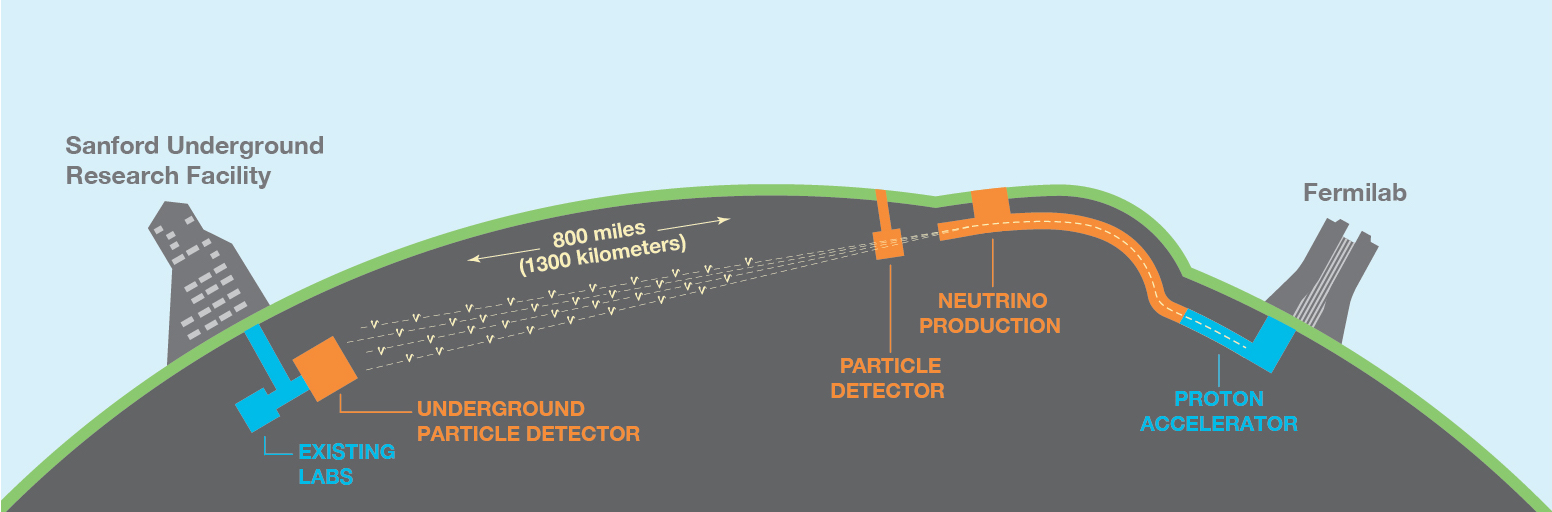
\includegraphics[width=\textwidth]{images/LBNE_Graphic_061615_2016.jpg}
\caption{Simple Draw up of DUNE FD taken from \citep{dune_cdr_2016_arxiv}}
\end{figure}

DUNE has three main science goals, all of which are geared towards pushing beyond the standard model:
\begin{itemize}
    \item Hadron Decay
    \item Neutrinos from Core-collapse supernovae
    \item Beamline neutrino interactions.
\end{itemize}

We will discuss the relevance of each of these items, and in \ref{chap:qpix} we will further discuss how the work presented here relates to each of these topics. 


Conventional horizontal drift detection for foreseeable DUNE modules are already considered possible for lengths up to 6.5m \citep{DUNE_Vertical:Paulucci_2022}.


\subsubsection{Hadron Decay}
\label{sect:intro_decay}

Second generation proton decay studies in the ICARUS experiment: \citep{ICARUS_2001}.

%% why do we care about hadron decay

\subsubsection{Supernova Studies}
\label{sect:intro_supernova}

%% why do we care about supernova neutrinos, what will they tell us?
The principal decay chain follows the pattern:
\begin{equation}
    \nu_{e} + ^{40}Ar \rightarrow e^- + ^{40}Kr^*
\end{equation}

%% text from the cdr 
% The neutrinos from a core-collapse supernova are emitted in a burst of a few tens of seconds
% duration, with about half the signal emitted in the first second. The neutrino energies are mostly
% 4The lifetime shown here is divided by the branching fraction for this decay mode, $\tau$ /B, and as such is a partial
% lifetime.
% Volume 1: The LBNF and DUNE Projects LBNF/DUNE Conceptual Design Report
% Chapter 2: DUNE Science 2–18
% in the range 5–50 MeV, and the luminosity is divided roughly equally between the three known
% neutrino flavors. Current experiments are sensitive primarily to electron antineutrinos ($\nu_e$), with
% detection through the inverse-beta decay process on free protons5
% , which dominates the interaction
%rate in water and liquid-scintillator detectors. Liquid argon has a unique sensitivity to the electronneutrino (νe) component of the flux, via the absorption interaction on 40Ar,

% This interaction can be tagged via the coincidence of the emitted electron and the accompanying
% photon cascade from the 40K∗ de-excitation. About 3000 events would be expected in a 40−kt
% fiducial mass liquid argon detector for a supernova at a distance of 10 kpc. In the neutrino channel
% the oscillation features are in general more pronounced, since the νe spectrum is always significantly
%different from the νµ (ντ ) spectrum in the initial core-collapse stages, to a larger degree than is
%the case for the corresponding ν¯e spectrum. Detection of a large neutrino signal in DUNE would
% help provide critical information on key astrophysical phenomena such as
%  the neutronization burst,
%  formation of a black hole,
%  shock wave effects,
%  shock instability oscillations, and
%  turbulence effects.
% In addition to yielding unprecedented information on the mechanics of the supernova explosion,
% the observation of a core-collapse supernova in DUNE will also probe particle physics, providing
% neutrino oscillation signatures (with sensitivity to mass hierarchy and “collective effects” due to
% neutrino-neutrino interactions), as well as tests for new physics such as Goldstone bosons (e.g.,
% Majorons), neutrino magnetic moments, new gauge bosons (“dark photons”), “unparticles” and
% extra-dimensional gauge bosons

%% what is the difference between NC and CC neutrino interactions.

\subsection{Pixelated Tracking Detectors}

\section{Even Further: Detectors in the Current Century}

Finally, in this last section we discuss recent development of various detector technologies.
There are many motivating pressures for new detectors to adopt pixelated designs. 
Below we discuss two contributing factors: the development of electronics and computing algorithms.

First, previously pixelated detectors have historically been more difficult because of the issues of cost and size regarding the number of readout channels.
This is being addressed, in part, by the advent of newer, cheaper, and larger Field-Programmable-Gate Arrays (FPGAs).
One method for reducing the electronic overhead required in pixelated detectors is to use digital multiplexing.
Cheap, high channel FPGAs directly solve this problem. 
Other electronics development, such as the Silicon-Photomultiplier, offer much cheaper alternatives for large pixel counters compared to their historical counter-parts. 

%% antihydrogen
\citep{Sadowski_2017}
Another driving factor is the the development of Machine Learning (ML) algorithms, particularly Convectional Neural Network (CNN \citep{Sadowski2017DeepLI}). 
Recent industry has driven the need for CNNs to be able to correctly identify and label 2-D images of various kinds, and thus championed much of progress in this field and spawned many kinds of CNN algorithms. 
%% cite sadowski here
Recently, it has been shown how these kinds of algorithms extend into High Energy Physics (HEP) for particle identification.
A major issue at the Intensity Frontier of physics is the sheer amount of data to store and process. 
These ML algorithms provied a developed tool to automate the analysis of huge amounts of data ($>> 1 TB$) and have been shown to be quite accurate ($>99\%$) at particle identification in LArTPCs.

%% LArPix / Argon Cube
\subsection{Current Pixelization Efforts in TPCs}

%% goeldi inspiration here from LArPix

Additional work has been performed in recent years which show that LArTPCs can also utilized a pixel-based readout \citep{larpix:Dwyer_2018}, \citep{Asaadi_2018}.

\subsection{SANDD}

Another Example of a pixelated detector is \citep{SUTANTO2021_sandd_165409}.


\subsection{The Single Volume Scatter Camera}

This work is presented in greater detail in (Appendicies-\ref{chap:OS1}/\ref{chap:OS2}) and represents a substantial amount of my own individual contribution. 
I am the 2nd author on the the paper described in Appendix-\ref{chap:OS1} and the corresponding author of Appendix-\ref{chap:OS2}, where I also collected and analyzed all presented data therein.

\subsection{Future Detectors}

The end of the Standard Model era is inevitable.
SM simply fails to account for physics with all major frontiers for physicists to accept its completeness; we know there is much and more to learn about nature.

The 20th century saw unprecented progress in its sophistication of its detectors from ray tubes, to spark chambers, to proportional counters, and to huge (>20 km) particle accelerators.
This century shows no signs holding any less promise than its predecessor.
Continued development in electronics, computing, and analysis methods will lead to more and newer frontiers of physics.

The work presented in this introduction aims to not only encapsulate the massive progress particle physics has made since the electron's discovery, but also to server as a reminder of how extraordinally surprising nature is.
At every turn and at every point where physicists think they've arrived at the end (or at an impossible roadblock) there always remains more to discover.
If we have learned anything, we have learned to knock and the door shall be opened.
